\documentclass[a4paper]{article}

%\usepackage{algorithm,amsmath,amssymb,subfig,url}
\usepackage{amsmath,amssymb,booktabs}
\usepackage[pdftex]{graphicx}
\usepackage[margin=30mm]{geometry}
%\usepackage[format=hang,labelfont=it]{caption}
%\usepackage[noend]{algorithmic}

%\floatname{algorithm}{Listing}
%\algsetup{indent=3em}
%\renewcommand{\algorithmiccomment}[1]{\quad \{\emph{#1}\}}



\begin{document}
\title{
  \large
  DT8014 Algorithms Group Activities (2014)\\
  \Large
  Week 4 -- Randomization}
\author{Roland Philippsen}
\maketitle



\noindent
Form groups of 4-5 students and work together on the following tasks.


%\section*{Neighboring Solutions}
%
%\emph{Purpose: first steps with exploring combinatorial solution spaces.}



\section*{Simulated Annealing (SA)}

\emph{Purpose: understand the basic SA iteration.}

\noindent
Consider the complete graph specified as the adjacency matrix below.
Assume you are trying to solve the TSP on this graph using SA.
The chosen transition probability function is

\begin{equation}
  P (f_i, f_j) = \begin{cases}
    1                     &\text{if}\; f_j < f_i \\
    \exp{\bigl((f_i - f_j) / T\bigr)} &\text{otherwise}
  \end{cases}
\end{equation}

\noindent
where $f_i$ is the cost of the current solution, $f_j$ the cost of the candidate solution, and $t$ is the temperature parameter.

\begin{itemize}
\item
  What is the probability of transitioning from \textbf{(A, C, B, D)} to \textbf{(A, C, D, B)} if the temperature is $T=10$?
\end{itemize}

\begin{center}
  \begin{tabular}{lrrrr}
    \toprule
      &  A &  B &  C &  D \\
    \midrule
    A &    &  8 &  5 &  6 \\
    B &  8 &    &  3 &  9 \\
    C &  5 &  3 &    &  7 \\
    D &  6 &  9 &  7 &    \\
    \bottomrule
  \end{tabular}
\end{center}

% don't forget to add the cost for closing the cycle!
%
% fi = 5+3+9+6 = 23
% fj = 5+7+9+8 = 29
%
% exp ((23 - 29) / 10) = exp (-0.6) = 0.548811636094



\section*{Genetic Algorithm (GA)}

\emph{Purpose: think about how to encode candidate solutions for GAs.}

\noindent
In the TSP, every vertex must be visited exactly once.
This is called a \emph{tour}.
In order to apply crossover, which is a fundamental components of GAs, it would thus be best to use an encoding that always corresponds to a tour.

In its basic form, the crossover operation takes two individuals from the current population, chooses a random crossover point, and swaps the encoding subsequence before and after this point.
Formally, let the sequence $(s_1 \ldots s_n)$ denote one of the individuals, and $(t_1 \ldots t_n)$ the other.
The crossover point $x$ is drawn e.g.\ from the uniform distribution, and the new sequences will be $(s_1 \ldots s_x, t_{x+1} \ldots t_n)$ and $(t_1 \ldots t_x, s_{x+1} \ldots s_n)$.

\begin{itemize}
\item
  Design an encoding, or modify the crossover operation, such the sequences are always tours.
\end{itemize}



\section*{Ant Colony Optimisation (ACO)}

\emph{Purpose: understand fundamental building blocks of ACO.}

\noindent
Consider the longest path problem on the graph in Figure~\ref{fig:aco}.
Assume ACO is being used, with a population size of two ants.
Initially, all edge pheromone levels are zero.
The pheromone update rule is simply that the ant with the longest weighted path deposits two units of pheromone on every edge it visited, whereas the other ant deposits only a single unit.

The basic exploration probability rule is given by

\begin{equation}
  P(u,v) = \frac{1 + p(u,v)}{\sum_{w \in N(u)} \bigl(1 + p(u,w)\bigr)}
\end{equation}

\noindent
where $u$ denotes the current vertex, $v$ and $w$ denote neighboring vertices, $N(u)$ is the set of vertices reachable from $u$, and $p(u,v)$ denotes the pheromone level of the edge $(u,v)$.

The ants have randomly initialized to the solutions \textbf{(F, G, E, B, C)} and \textbf{(A, D, E, C, B)}.

\begin{enumerate}

\item
  What are the pheromone levels that result from these paths?

\item
  After the pheromone update you just computed, what is the value of $P(E,B)$ -- the probability of going from vertex E to B?
  And how high is $P(B,E)$?

  % weight sum of ant a: 11+9+7+8 = 35
  % ant b:               5+15+5+8 = 33
  %
  % ant a depostits 2 pheromone units on edges FG, GE, EB, and BC
  % ant b deposits 1 unit on edges AD, DE, EC, CB
  %
  % edge BC (and CB) occur in both paths, it ends up with value 3
  % edges FG, GE, EB end up with 2 units each
  % edges AD, DE, EC with 1 unit
  %
  % from E to B: (1 + 2) / (5 + 2x2 + 2x1) = 3 / 11 = 0.273
  % from B to E: (1 + 2) / (4 + 2 + 3)     = 3 / 9  = 0.333
  
\item
  In the longest path problem, a vertex can be visited at most once.
  Formulate a complete exploration step such that this constraint is not violated?
  
\end{enumerate}

\begin{figure}
  \centering
  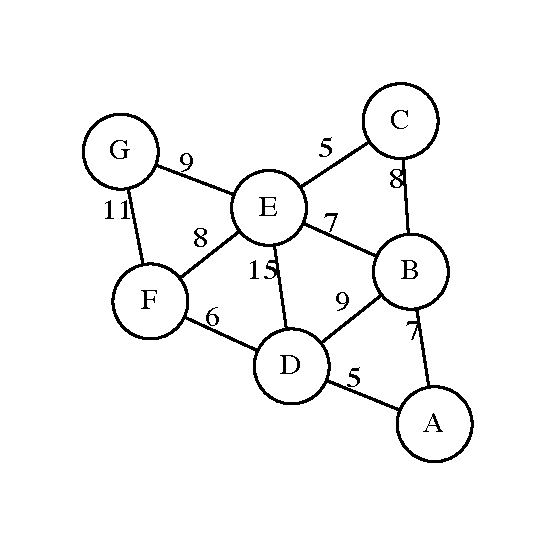
\includegraphics[width=0.4\columnwidth,trim=1cm 1cm 1cm 1cm]{fig/mst-exercise-1.pdf}
  \caption{
    Example weighted undirected graph.
  }\label{fig:aco}
\end{figure}

\end{document}
